\documentclass[final]{beamer}
\usepackage{grffile}
\mode<presentation>{\usetheme{BDigital}}
\usepackage[english]{babel}
%\usepackage[latin1]{inputenc}
\usepackage{amsmath,amsthm, amssymb, latexsym}
\usepackage{multirow}
\usepackage{algorithm}
\usepackage{algpseudocode}
\usepackage{latexsym}
\usepackage{xcolor}
%\usepackage{times}\usefonttheme{professionalfonts}  % obsolete
%\usefonttheme[onlymath]{serif}
\boldmath
\usepackage[orientation=portrait,size=a0,scale=1.4,debug]{beamerposter}
% change list indention level
% \setdefaultleftmargin{3em}{}{}{}{}{}


%\usepackage{snapshot} % will write a .dep file with all dependencies, allows for easy bundling

\usepackage{array,booktabs,tabularx}
\newcolumntype{Z}{>{\centering\arraybackslash}X} % centered tabularx columns
\newcommand{\pphantom}{\textcolor{ta3aluminium}} % phantom introduces a vertical space in p formatted table columns??!!

\listfiles

%%%%%%%%%%%%%%%%%%%%%%%%%%%%%%%%%%%%%%%%%%%%%%%%%%%%%%%%%%%%%%%%%%%%%%%%%%%%%%%%%%%%%%
\graphicspath{{figures/}}
 
\title{\huge Pruning AdaBoost for Continuous Sensors Mining Applications}
\author{Mojdeh Rastgoo, Guillaume Lemaitre, Xavier Rafael, Felip Miralles and Pier Luigi Casale}
\institute[BDigital Technology Centre]{eHealth R\&D, BDigital Technology Centre, Barcelona, Spain}
\date[Aug. 27th, 2012]{Aug. 27th, 2012}

%%%%%%%%%%%%%%%%%%%%%%%%%%%%%%%%%%%%%%%%%%%%%%%%%%%%%%%%%%%%%%%%%%%%%%%%%%%%%%%%%%%%%%
\newlength{\columnheight}
\setlength{\columnheight}{105cm}


%%%%%%%%%%%%%%%%%%%%%%%%%%%%%%%%%%%%%%%%%%%%%%%%%%%%%%%%%%%%%%%%%%%%%%%%%%%%%%%%%%%%%%
\begin{document}
\begin{frame}
  \begin{columns}
    % ---------------------------------------------------------%
    % Set up a column 
    \begin{column}{.49\textwidth}
      \begin{beamercolorbox}[center,wd=\textwidth]{postercolumn}
        \begin{minipage}[T]{.95\textwidth}  % tweaks the width, makes a new \textwidth
          \parbox[t][\columnheight]{\textwidth}{ % must be some better way to set the the height, width and textwidth simultaneously
            % Since all columns are the same length, it is all nice and tidy.  You have to get the height empirically
            % ---------------------------------------------------------%
            % fill each column with content            
            \begin{block}{Introduction}
              \begin{itemize}
               \item Crucial task of mining sensors data in continuous learning environment               
               \item AdaBoost is a well known framework for mining continuous streams, however when many subsequent batches of data are provided, AdaBoost tends to create large ensembles that suffer of two main drawbacks: 
               \begin{itemize}               
               \item Increasing memory 
               \item Over-fitting 
               \end{itemize}
               \item Pruning techniques for AdaBoost classifier considering continuous learning environment could provide: 
                \begin{itemize}
                \item Least memory consuming ensembles for each stage of learning  
                \item A first attempt to retain only the significant information acquired from previous knowledge
                \end{itemize}
                \end{itemize}
%              \item We propose/analyze:
%                \begin{itemize}
%                \item grid-based and dense extraction of local features
%                \item block-based matching accounting for different\\
%	                  viewpoints and registration errors
%                \end{itemize}
%              \end{itemize}              
            \end{block}
            \vfill
%            \begin{block}{AdaBoost}
%            \begin{itemize}
%            \item Adaptive Boosting is an ensemble learning, which allows to achieve high performance with combination of weak learners.
%            \end{itemize}
%%              \begin{columns}
%%                \begin{column}{.55\textwidth}
%                \begin{algorithm}[H]
%                \vspace{2ex}
%				\caption{AdaBoost Algorithm}
%				\label{alg:adaBoost}
%				\floatname{algorithm}{Procedure}
%				\renewcommand{\algorithmicrequire}{\textbf{Input:}}
%				\renewcommand{\algorithmicensure}{\textbf{Output:}}
%				\algnewcommand\algorithmicinitialize{\textbf{Initialize}}
%				\algnewcommand\Initialize{\item[\algorithmicinitialize]}
%				\begin{algorithmic}
%				\footnotesize
%				\color{black}
%				\Require
%				\State - Training set of $N$ samples $(\mathbf{x}_{i} , y_{i})$, with $i=1 \dots N$, $\mathbf{x}_{i} \in R^{N}$ , $y_{k} \in Y = \{−1, +1\}$ ;
%				\State - Weak learning algorithm \textit{WeakLearn} ;
%				\State - Number of learning iteration $T$ ;
%				\State
%				\Initialize $W_{1}(k) = 1/N, k=1,\dots,N$ ;
%				\State
%				\For{$t=1,\dots,T$}
%				\State
%				\State 1. Train \textit{WeakLearn} using distribution $W_{t}$ and get weak hypothesis $\mathit{h}_{t}$ ;
%				\State 2. Compute classification error $\epsilon_{t} = Pr_{k \sim W_{t}}[h_{t}(x_{k})\neq y_{k}]$ ;
%				\State 3. Compute $\alpha_{t} = \frac{1}{2} \ln(\frac{1-\epsilon_{t}}{\epsilon_{t}})$ ;
%				\State 4. Update distribution: 
%				\begin{itemize}
%				\footnotesize
%	 			\item[]~~~~~~~~~~$W_{t+1}(k) = \frac{W_{t}(k) \exp(-\alpha_{t} y_{k} h_{t}(x_{k}))}{Z_{t}}$ ;
%	 			\item[]~~~~~~~~~~where $Z_{t}$ is a normalization factor chosen so that $W_{t+1}$ will be a proper distribution function.
%				\end{itemize} 
%				\EndFor
%				\State
%				\Ensure
%				\State $H(x) = \mbox{sign} (\sum_{t=1}^{T} \alpha_{t} h_{t}(x))$ ;
%				\end{algorithmic}
%				\end{algorithm}
%%                \end{column}
%%                \begin{column}{.44\textwidth}
%%        
%%                \end{column}
%%              \end{columns}
%             % \vskip-1ex
%            \end{block}
          \vfill
          \begin{block}{Reduce Error Algorithm (RE)}
              \begin{itemize}
              	\item New version of reduced error method introduced first by \textit{Margineantu \& Dietterich et el} 
              	\item Our implementation is different from the initial version since: 
              	\begin{itemize}
              		\item No back-fitting is performed after each selection
              		\item The selected classifiers are re-weighted based on the pruning distribution 
              	\end{itemize}
              \item RE algorithm:              
              	\begin{itemize}
              	\item Training AdaBoost on training set with 100 base classifiers $H$ 
              	\item The pruning distribution $W_{t}$ is initialized
              	\item The weak learner $h_{t}$ with minimum error on $W_{t}$ is added as first base classifier to $P$ while its weight $\alpha_{t}$ is updated.  Pruning distribution is updated as well $W_{t+1}$
             	\item For the desired number of base classifier, 
             	\begin{itemize}
              		\item The error of combination of each remaining classifier $h_{t}$ and $P$ is evaluated on $W_{t+1}$. The base classifier which leads to minimum error is added to $P$ and its relative weight $\alpha_{t}$ is updated
              	\end{itemize}
              	\end{itemize}
              \end{itemize}              
          \end{block}
            \vfill
          \begin{block}{Learner Weights Analysis (LWA)}
            \begin{itemize}
            		\item Distribution of weights (right) and learners (left) based on different dimension provided by AdaBoost for breast datasets
            		\begin{center}
     
              	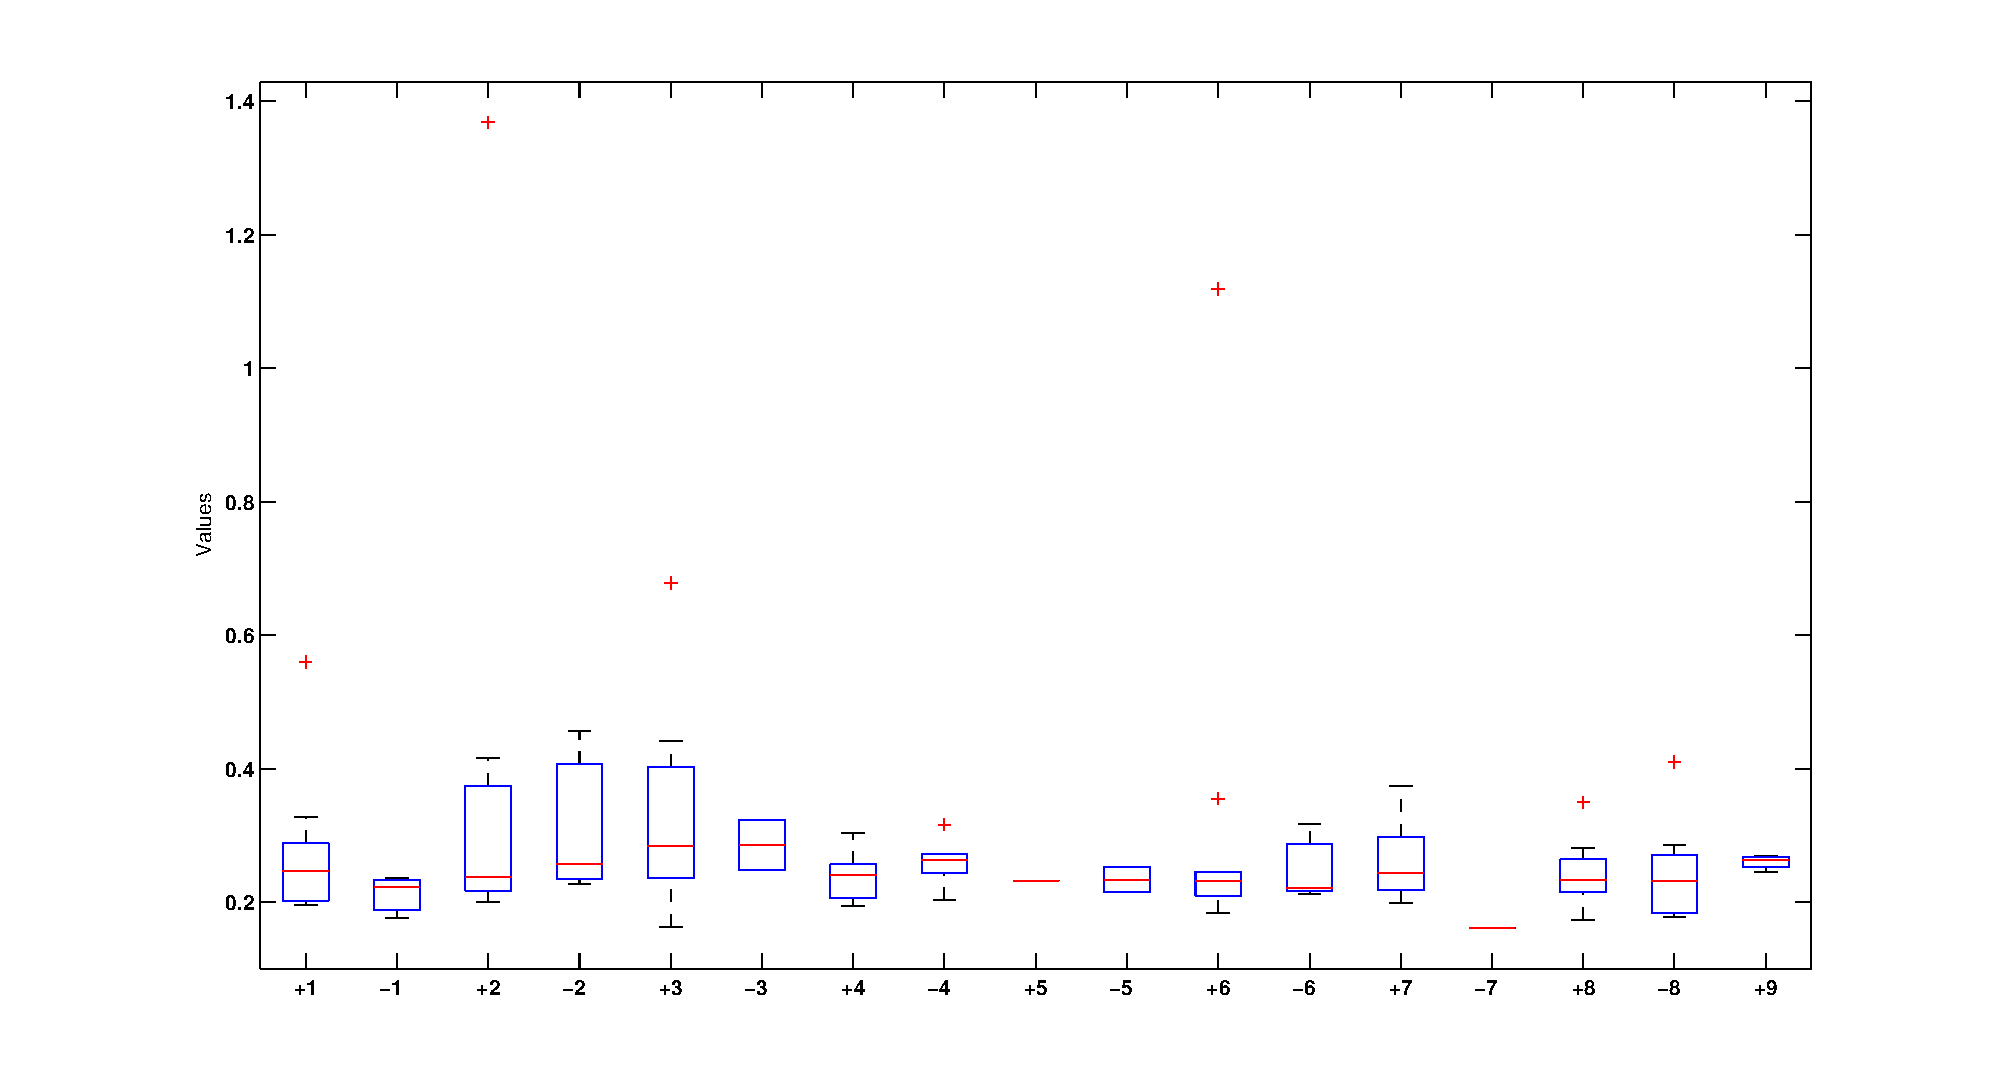
\includegraphics[width=0.45\linewidth]{images/drifts/breast_weights-eps-converted-to}
              \-
				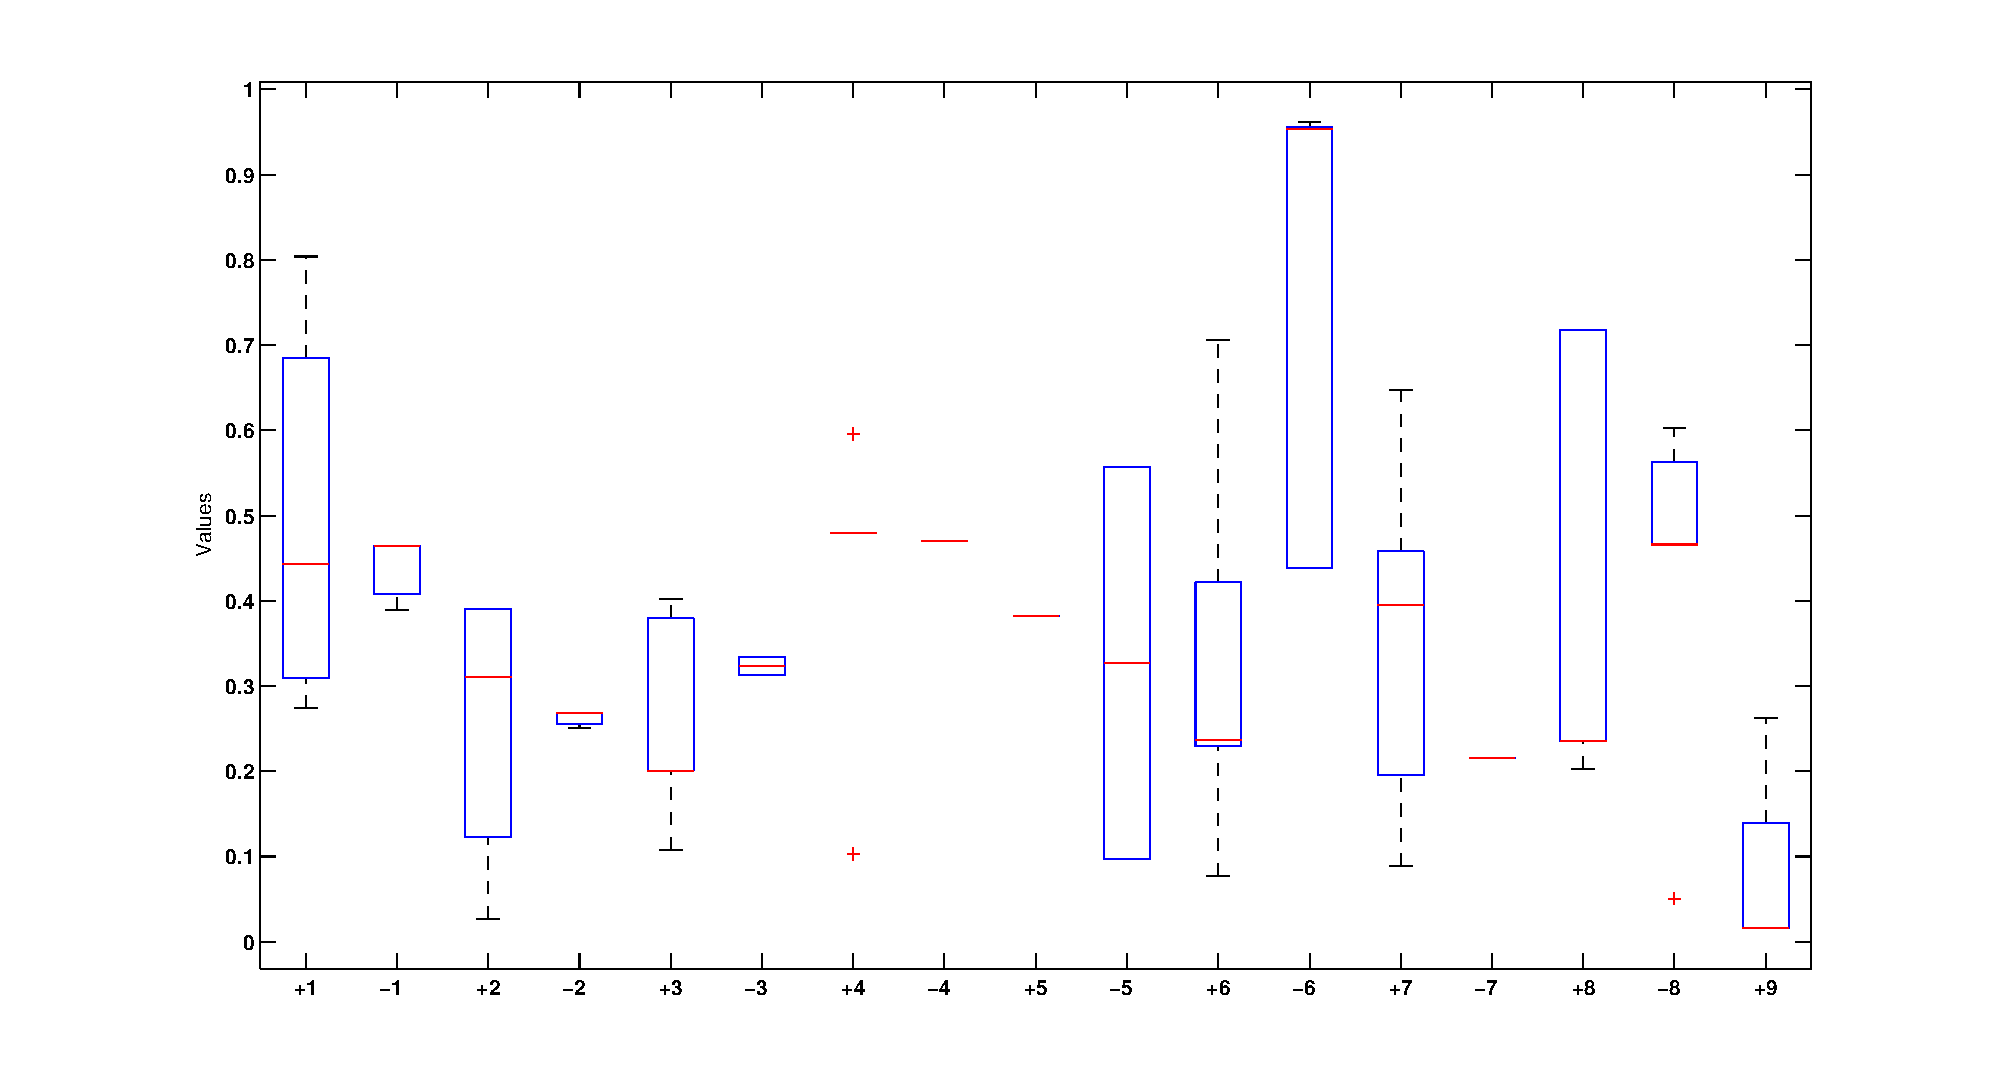
\includegraphics[width=0.45\linewidth]{images/drifts/breast_threshold-eps-converted-to}
			       
            		\end{center}
				\item Selection of weak learners based on the weight distribution considering: 
				\begin{itemize}
					\item Learners with higher weights have more impact
					\item An ensemble is better when more diversified the classifiers forming it are
				\end{itemize}
				\item LWA Algorithm: 
				\begin{itemize}
				\item The AdaBoost is trained on training set, providing $T$ decision stump classifier 
				\item The weights of decision stumps $\alpha_{t}$ are grouped using their dimension parameters (Matrix $M$ of size $n \times D$, when $n$ is the number of elements for each of $D$ dimensions)		 
				\item $M$ is sorted by row in descendant order, then sorted by column in a descendent order 
				\item Sorted $M$ is transformed to vector $V$ by concatenating the column of $M$
				\item $t$ first classifier corresponding to the first $t$ element of $V$ are selected for final ensemble 
			
				\end{itemize}
            \end{itemize}  
          \end{block}
          \begin{block}{Pareto Analysis (PA)}
          	\begin{itemize}
          		\item PA is based on the assumption that few key actions will produce significant overall effects 
          		\item This technique estimates the effectiveness of each feature dimension and accordingly selects the classifier from feature dimensions with higher impact
          		\item The effectiveness could be adjusted based on threshold
          		\item This method could work in an automatic way, where only few classifier will be selected based on their effectiveness, or in an non-automatic way the number of desired classifiers are fixed
%          		\item PA Algorithm: 
%          		\begin{itemize}
%          			\item The features are grouped based on total number of weights outliers in each. 
%          			\item The frequency distribution of outliers are sorted in descendant order.
%          			\item The cumulative percentage of the sorted group is computed.
%          			\item All the dimensions with lower cumulative error than the specified threshold are considered.
%          		\end{itemize}
         	\end{itemize}            
               
          \end{block}
            \vfill
           
          }
        \end{minipage}
      \end{beamercolorbox}
    \end{column}
    % ---------------------------------------------------------%
    % end the column

    % ---------------------------------------------------------%
    % Set up a column 
    \begin{column}{.49\textwidth}
      \begin{beamercolorbox}[center,wd=\textwidth]{postercolumn}
        \begin{minipage}[T]{.95\textwidth} % tweaks the width, makes a new \textwidth
          \parbox[t][\columnheight]{\textwidth}{ % must be some better way to set the the height, width and textwidth simultaneously
            % Since all columns are the same length, it is all nice and tidy.  You have to get the height empirically
            % ---------------------------------------------------------%
            % fill each column with content
			\begin{block}{Pareto Analysis (PA)}
			\begin{itemize}		
			\item PA Algorithm: 
          		\begin{itemize}
          			\item The features are grouped based on total number of weight outliers in each of them 
          			\item The frequency distribution of outliers are sorted in descendant order
          			\item The cumulative percentage of the sorted group is computed
          			\item All the dimensions with lower cumulative error than the specified threshold are considered
          		\end{itemize}
          			
			\end{itemize}
			
			\end{block}
            \begin{block}{Results: UCI Datasets Repository}
              \begin{itemize}
              \item 10-fold cross-validation on 14 UCI datasets - 90\% pruning
              \end{itemize}
              \vskip-0.5ex
              \centering
              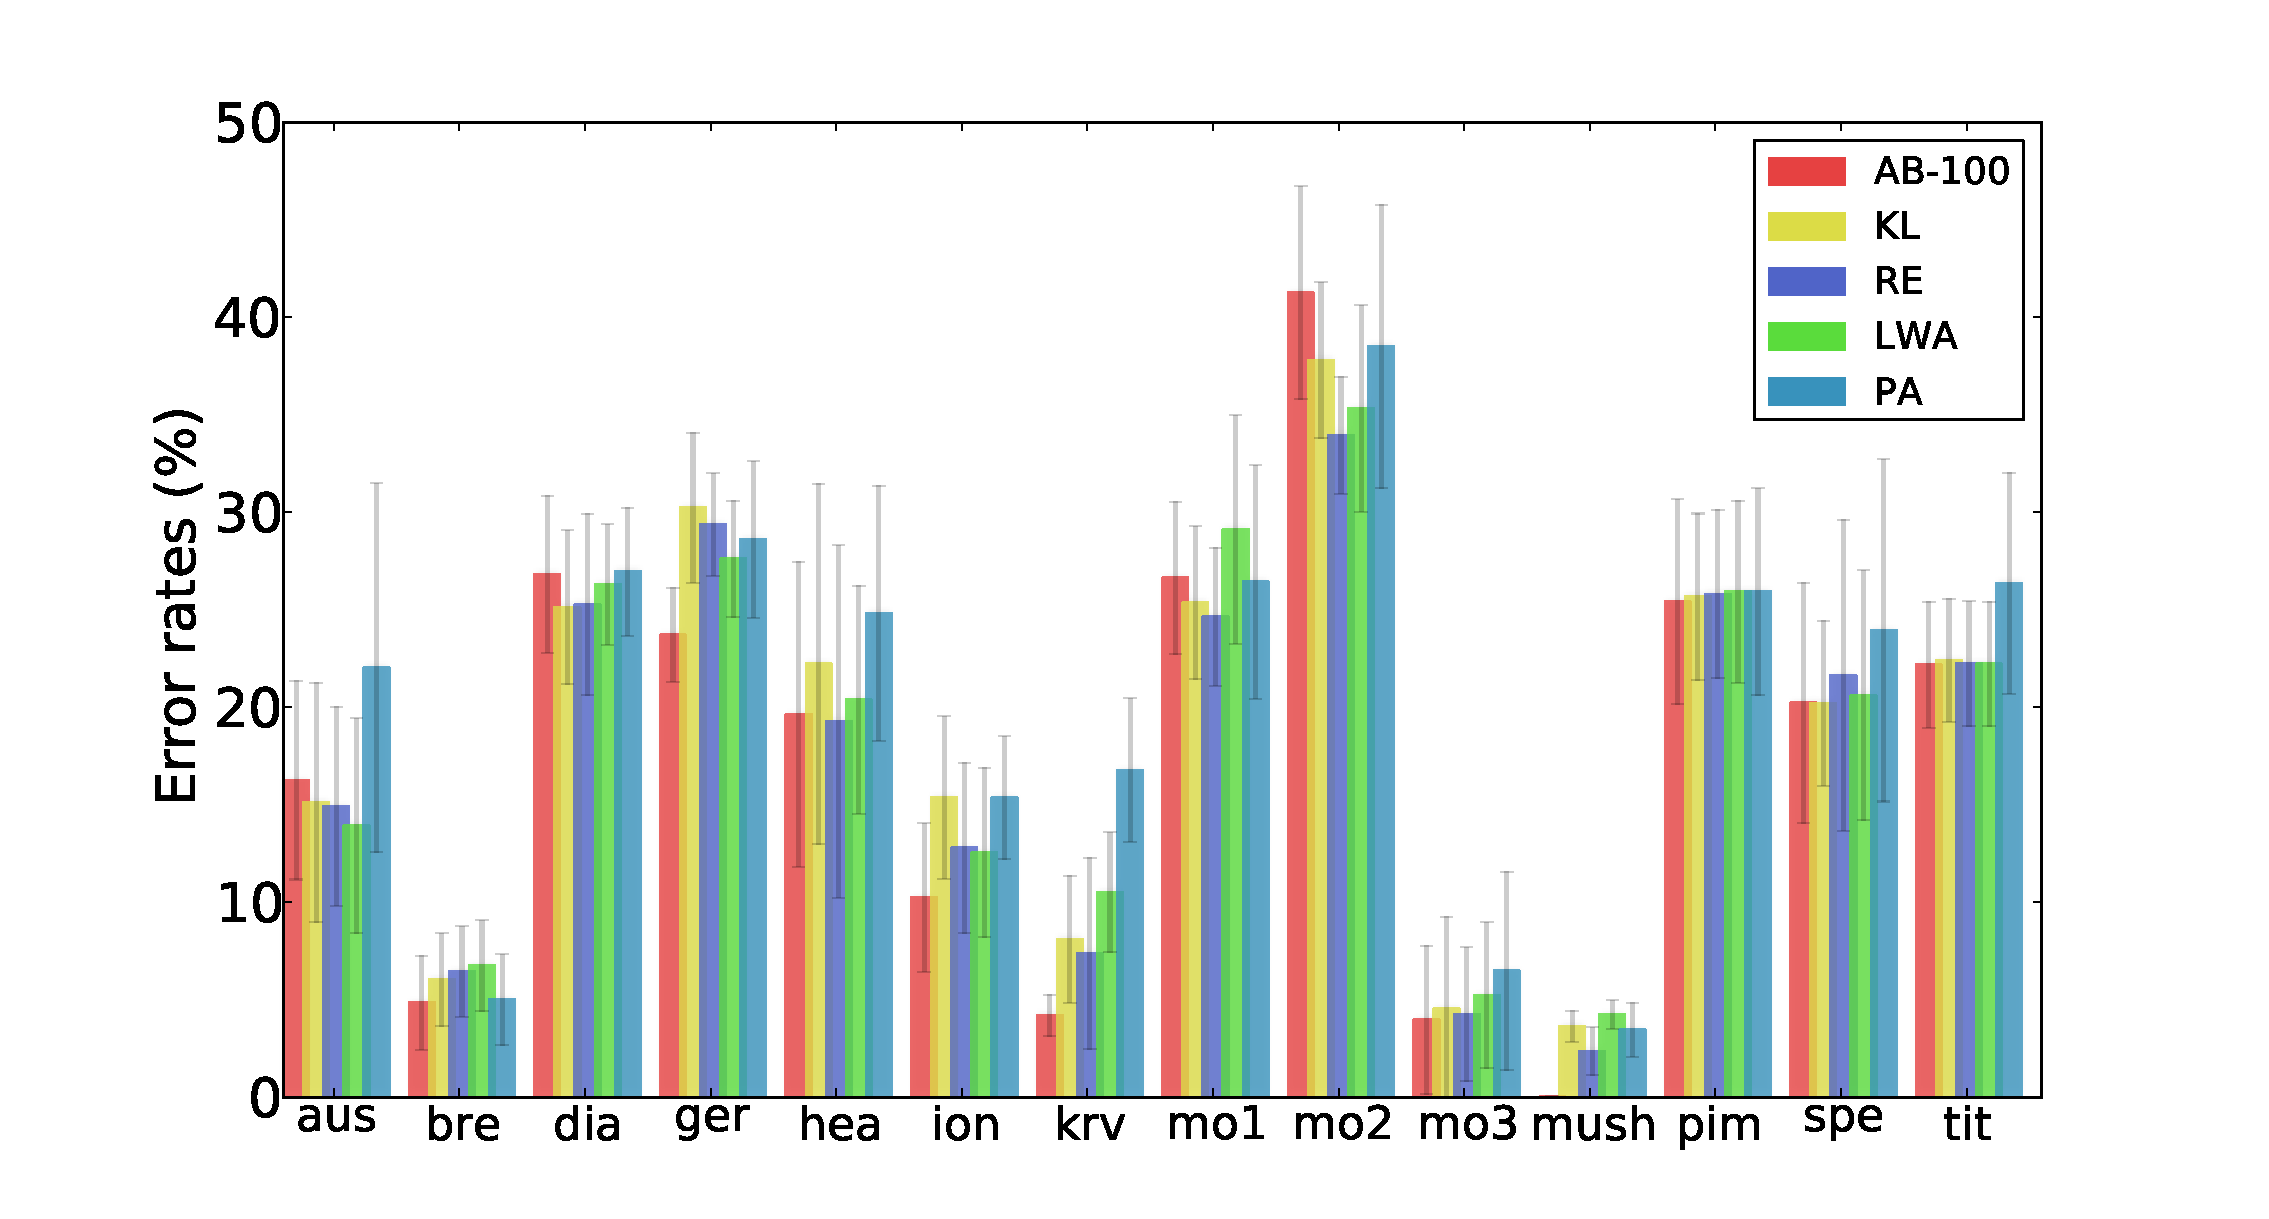
\includegraphics[width=0.8\linewidth]{results/uci/extended/resultUCI}
            \end{block}
            \vfill
            \begin{block}{Results: Simulated Drifting Datasets}
            \begin{itemize}
              		\item Simulated drifts datasets, Dataset~1, linear drift (right), Dataset~2, circular drift (middle), Dataset~3, circular drift (left)
	             \end{itemize}
			\centering
			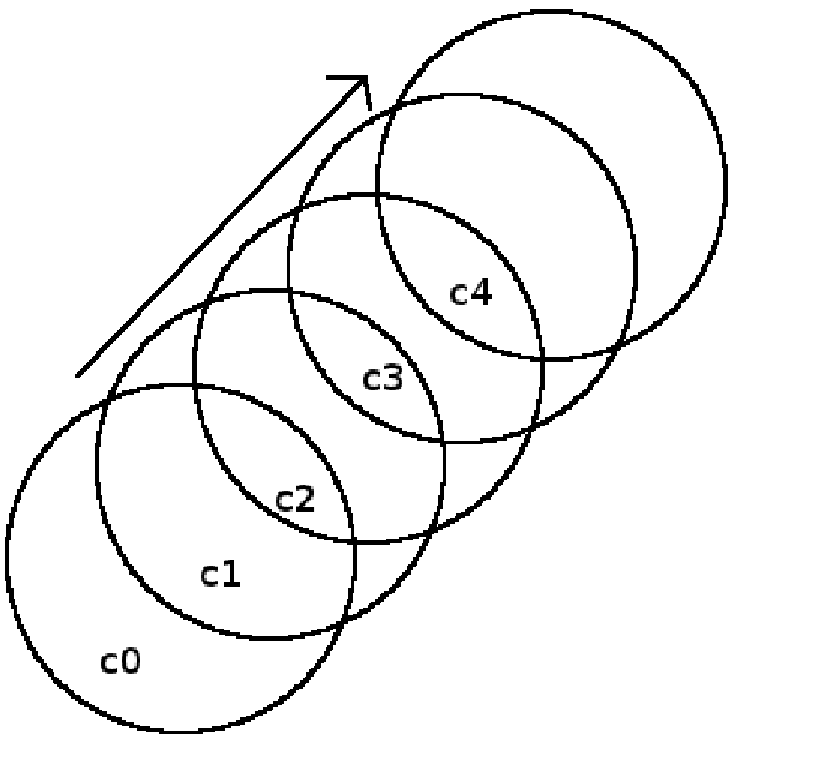
\includegraphics[width=0.2\linewidth]{images/drifts/Line-eps-converted-to}
			 \-
			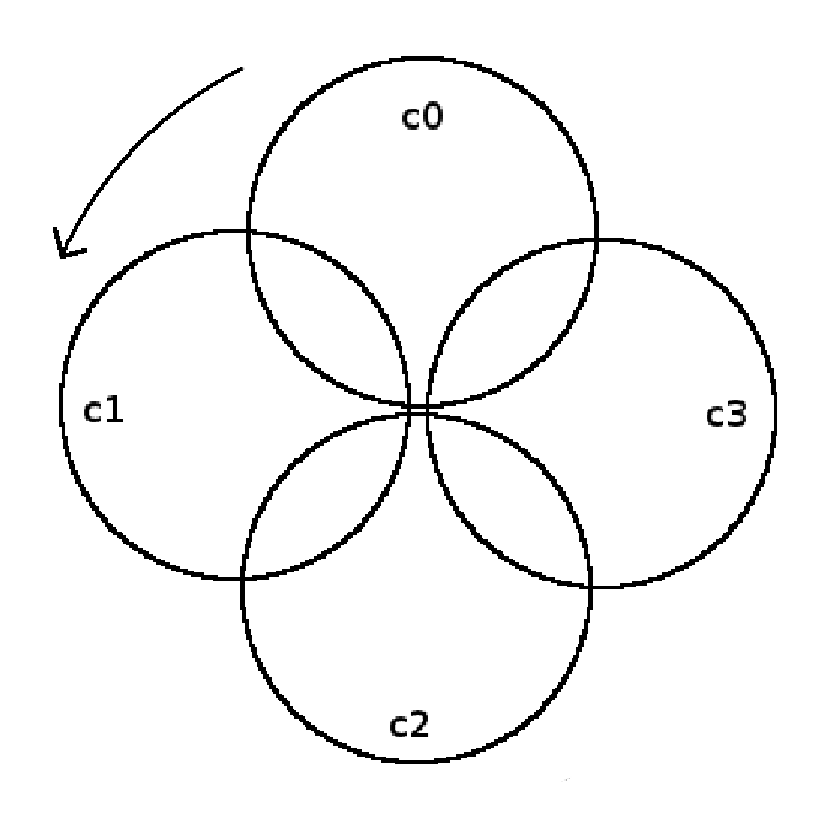
\includegraphics[width=0.2\linewidth]{images/drifts/circle_2share-eps-converted-to}
			 \-
			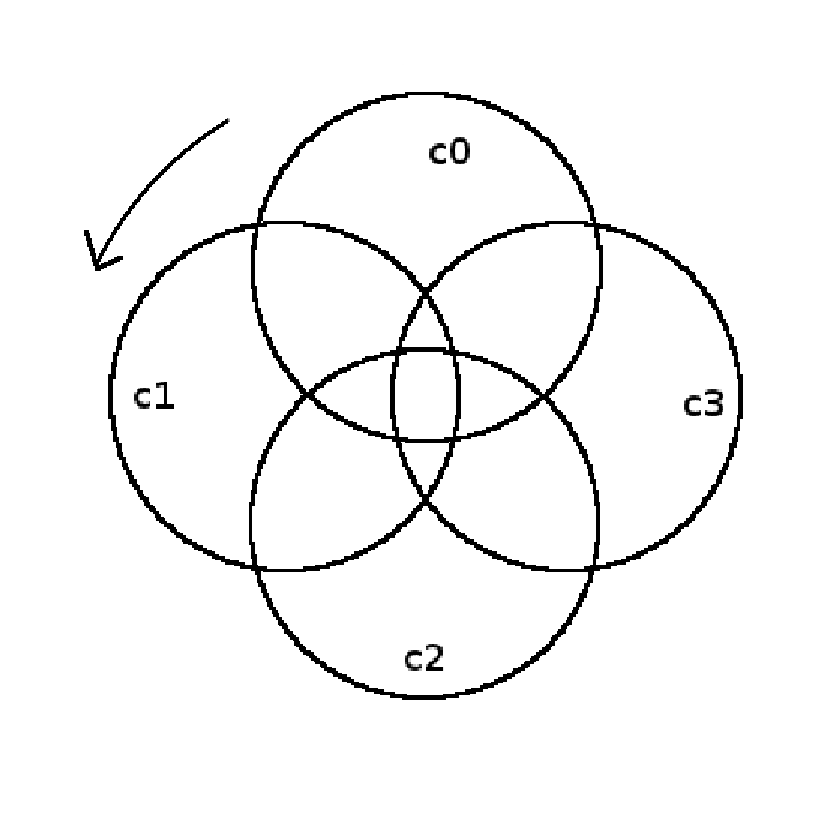
\includegraphics[width=0.2\linewidth]{images/drifts/circle_4share-eps-converted-to}
				\begin{itemize}
              		\item Exp. 1, Goal: Classifying final stage of data
	             \end{itemize}
              	 \centering
              	 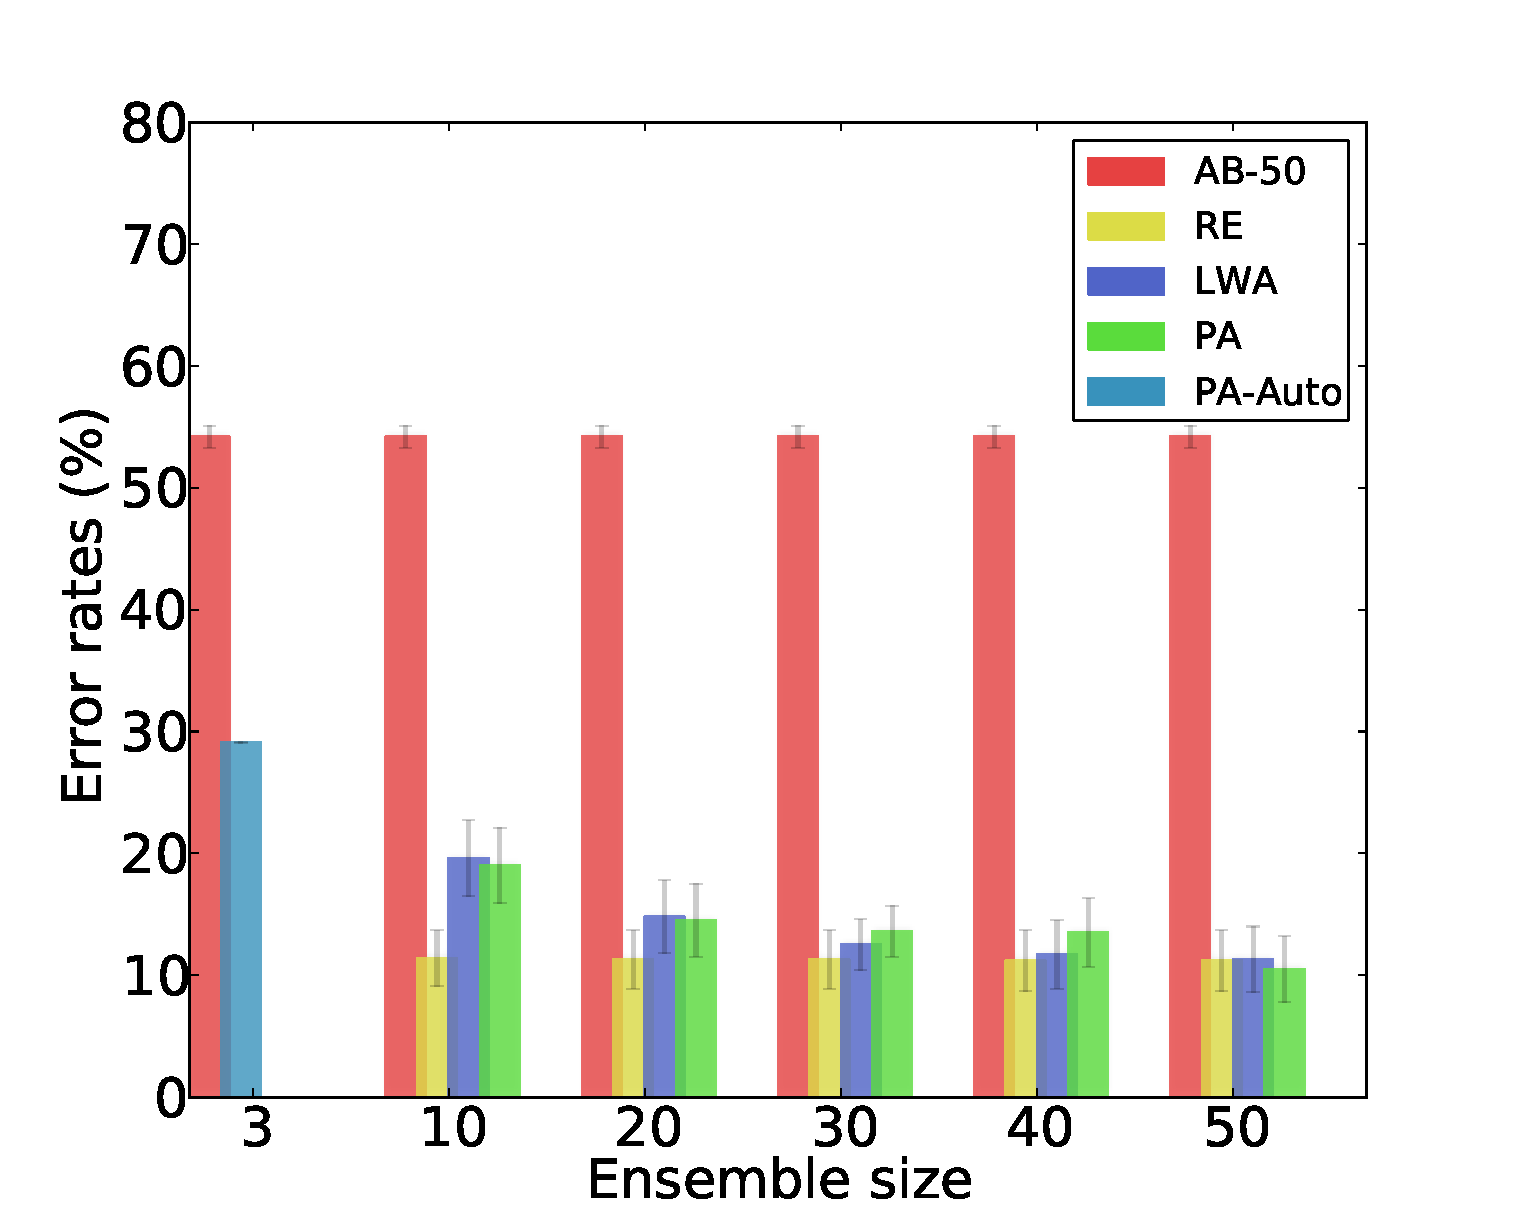
\includegraphics[width=0.3\linewidth]{results/drifts/extended/resultArtificial1Pool}
                  \-
                  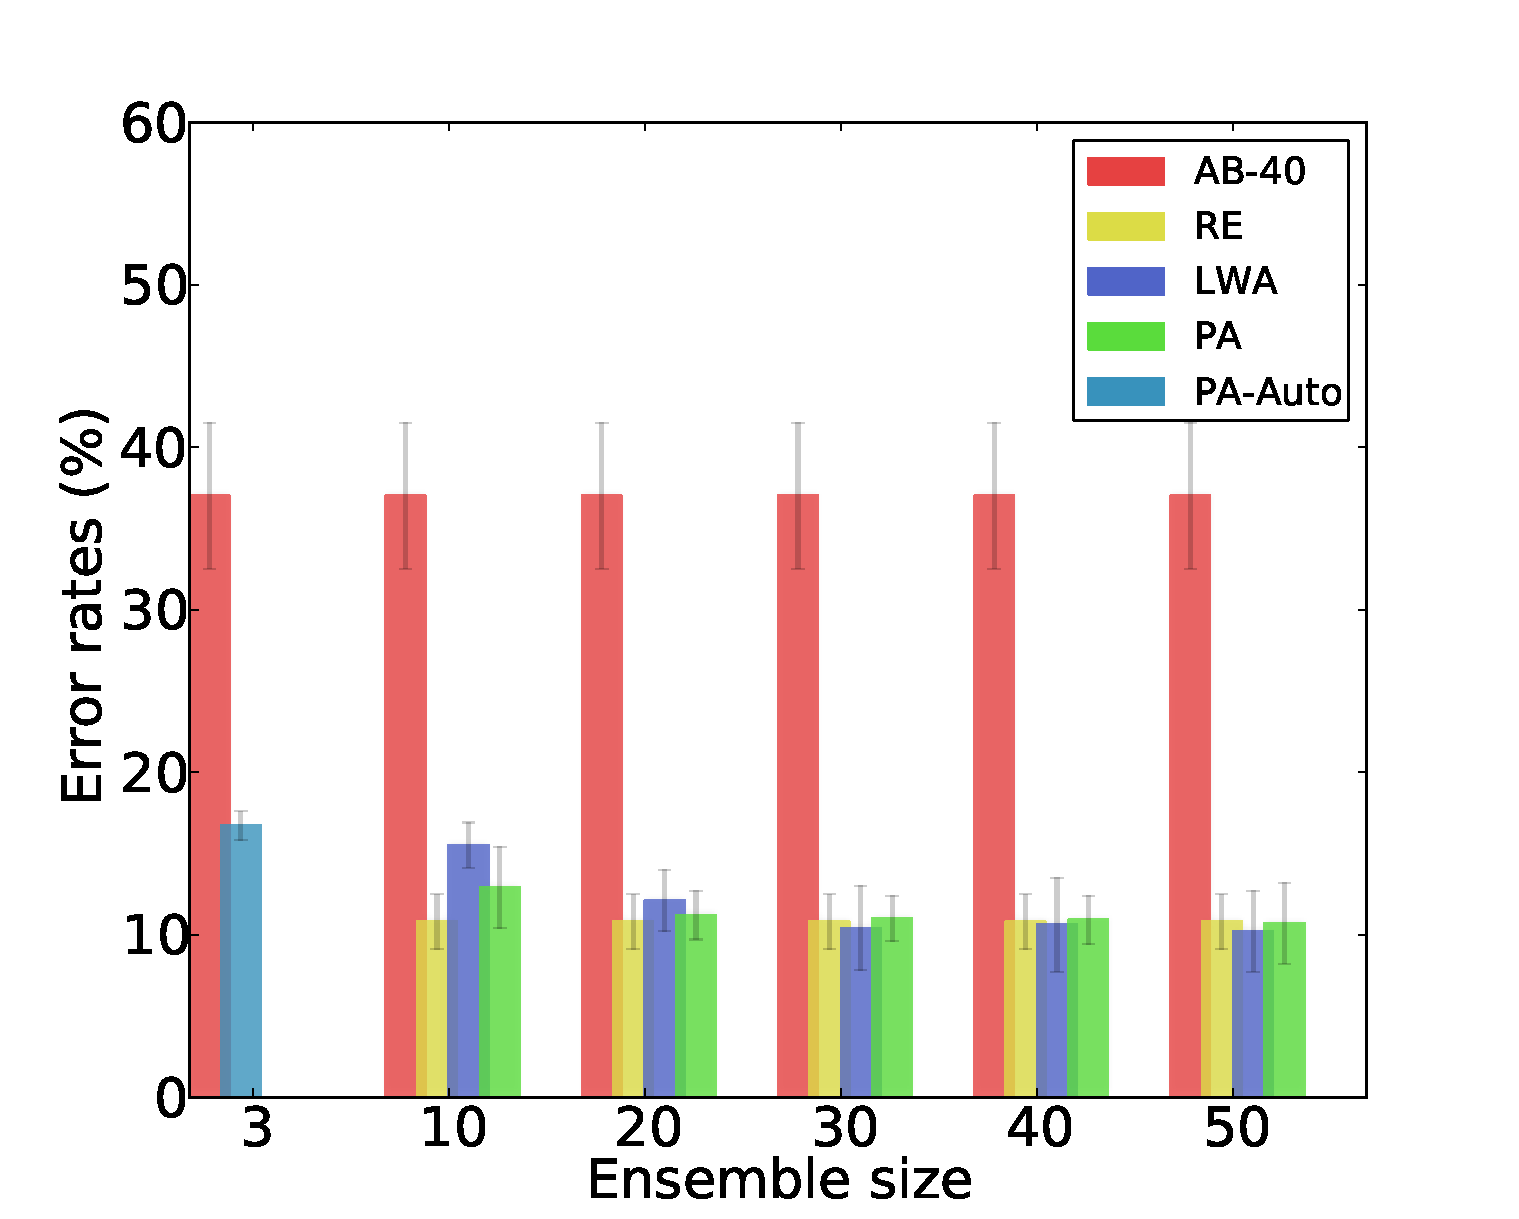
\includegraphics[width=0.3\linewidth]{results/drifts/extended/resultArtificial2Pool}
                  \-
                  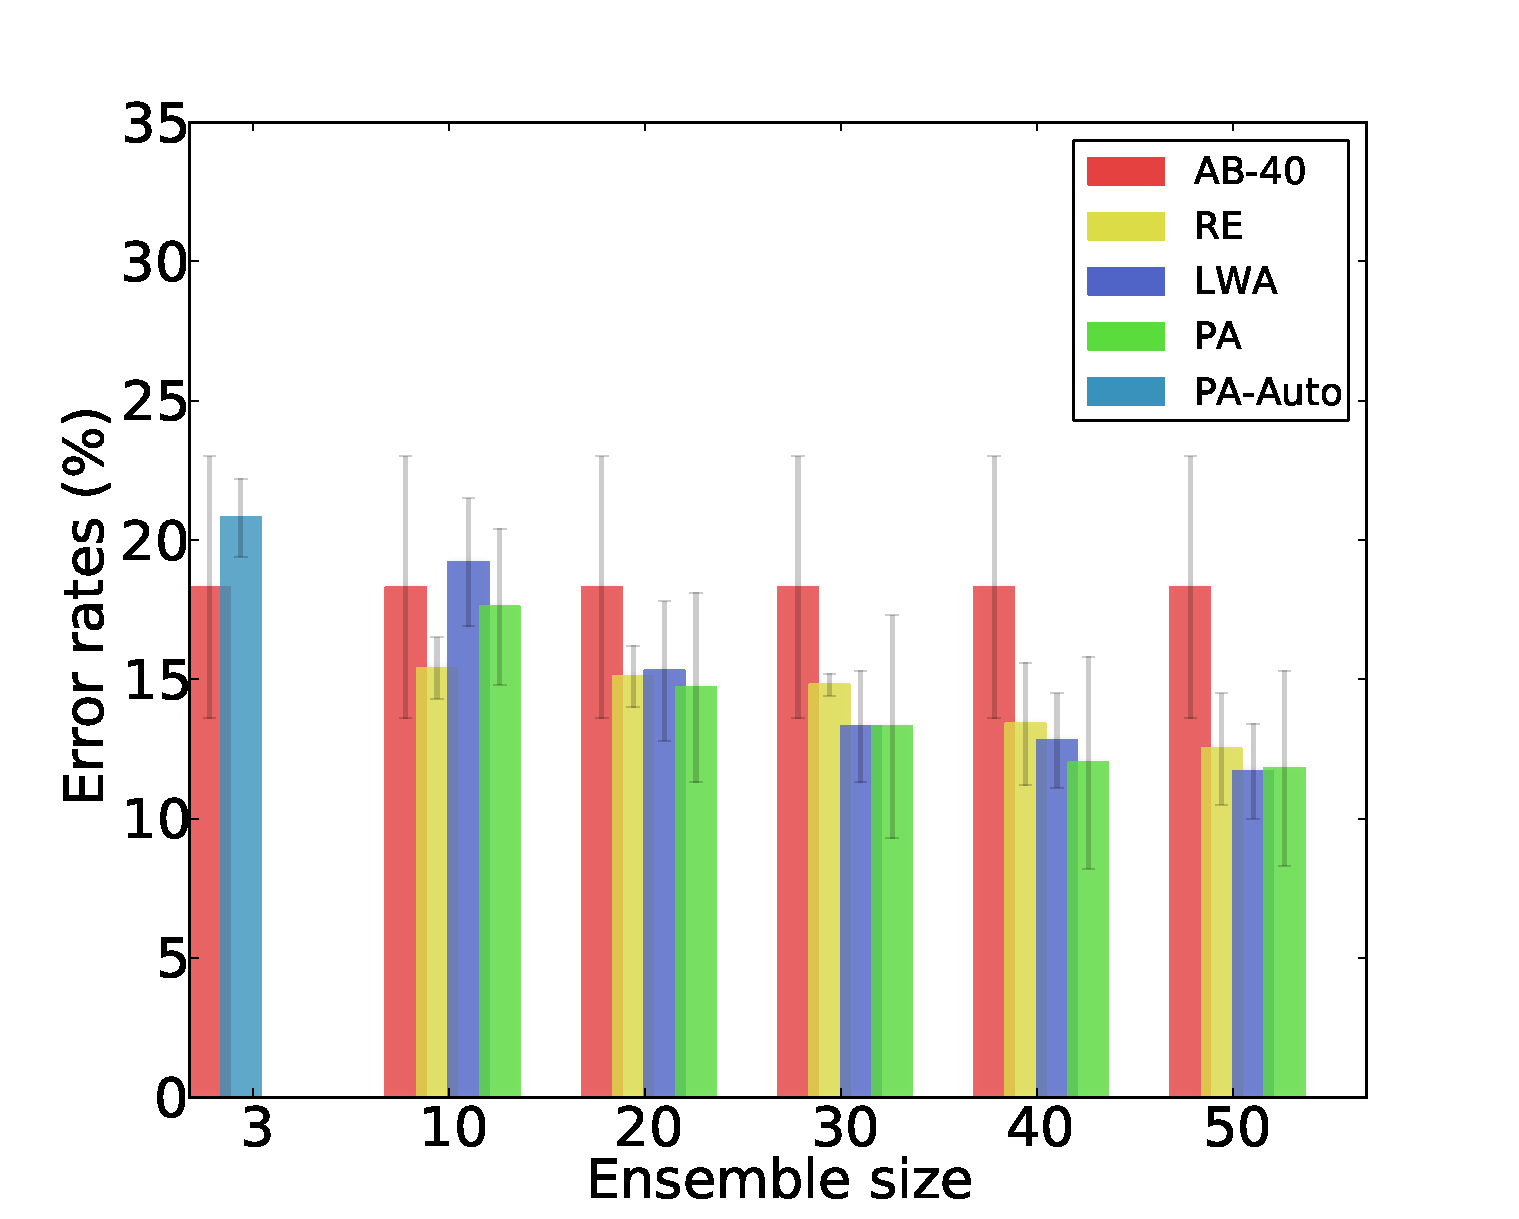
\includegraphics[width=0.3\linewidth]{results/drifts/extended/resultArtificial3Pool}
                  \begin{itemize}
              		\item Exp. 2, Goal: Classifying whole datasets (keeping memory of previous stages)
	             \end{itemize}
				 \centering
                  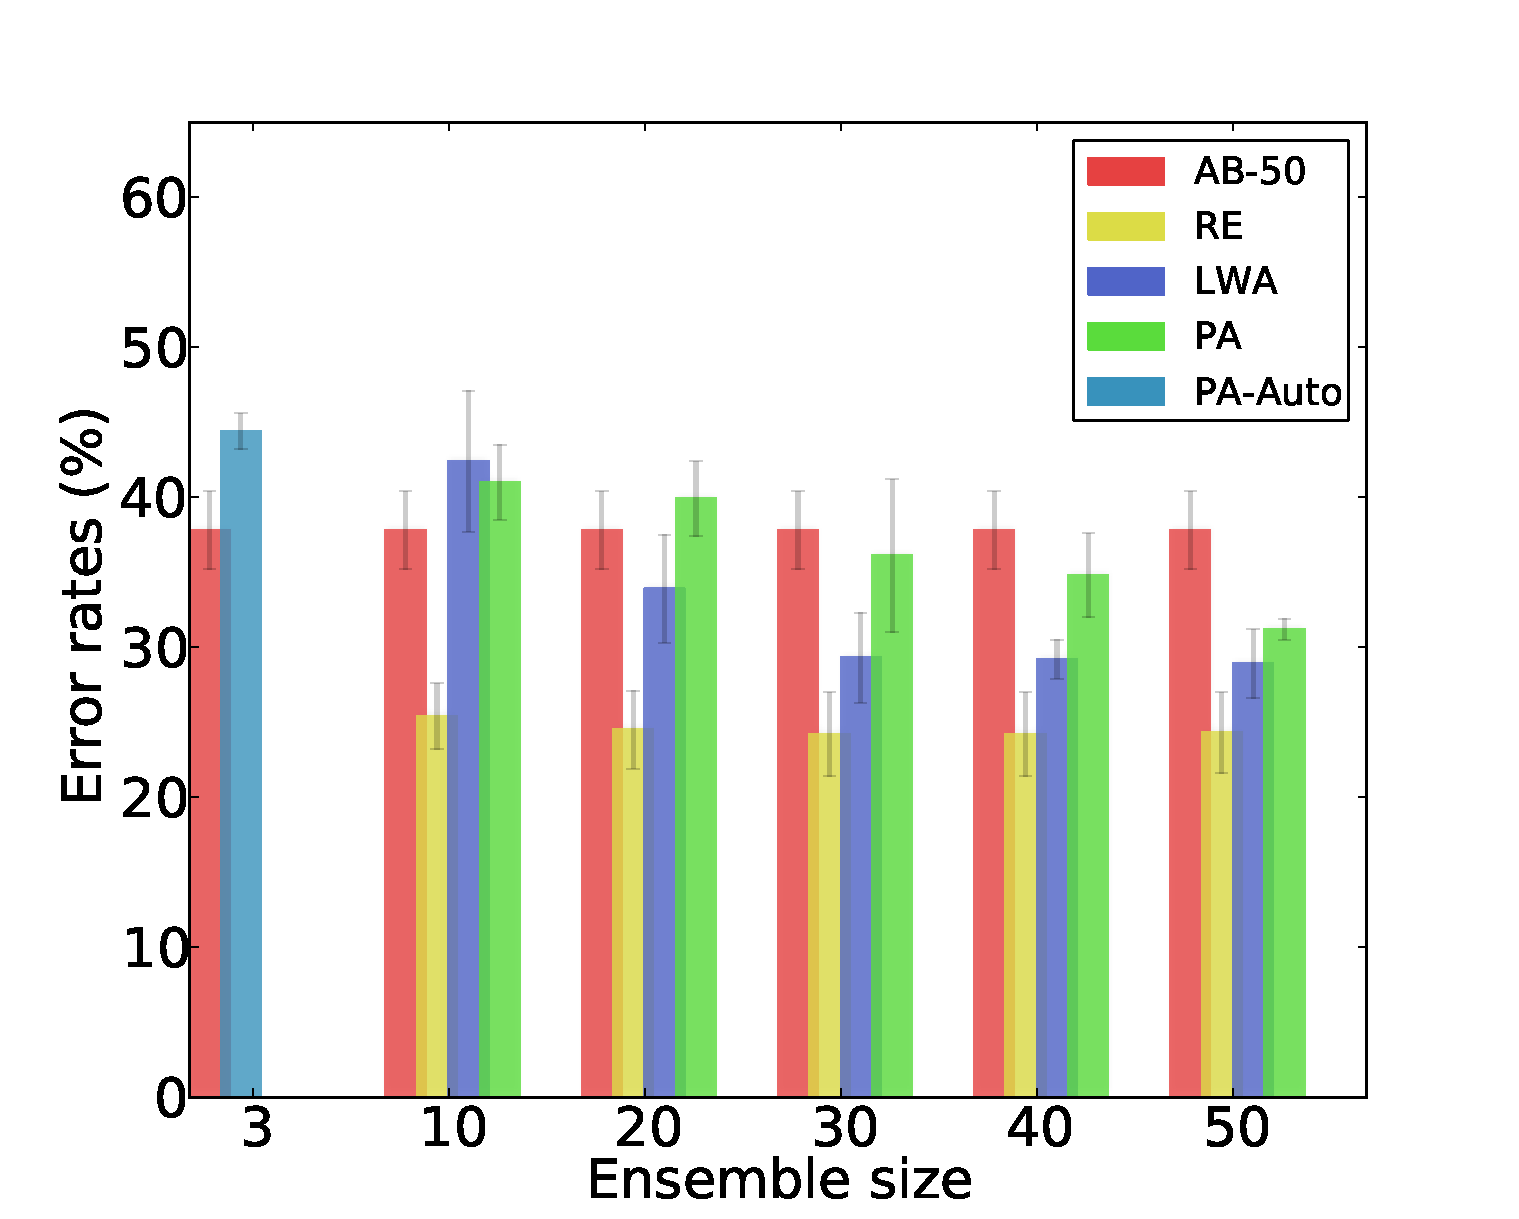
\includegraphics[width=0.3\linewidth]{results/drifts/extended/resultArtificial1MemPool}
                  \-
                  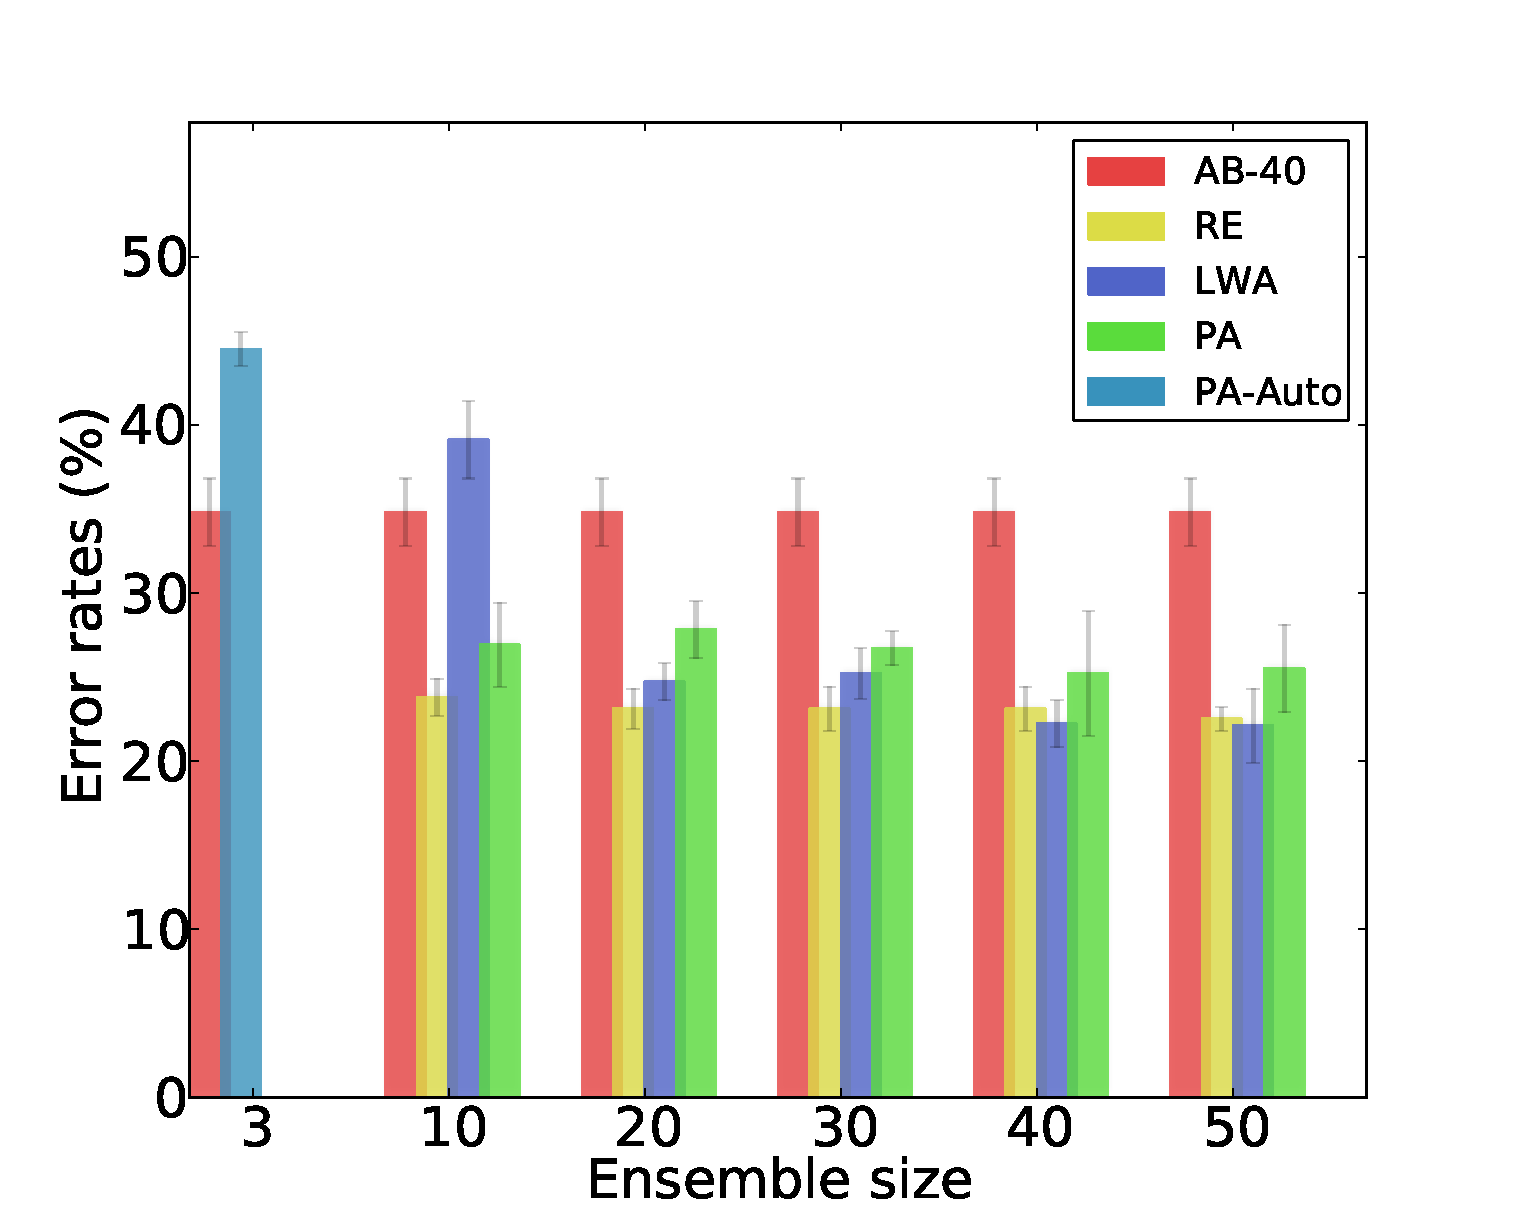
\includegraphics[width=0.3\linewidth]{results/drifts/extended/resultArtificial2MemPool}
                  \-
                  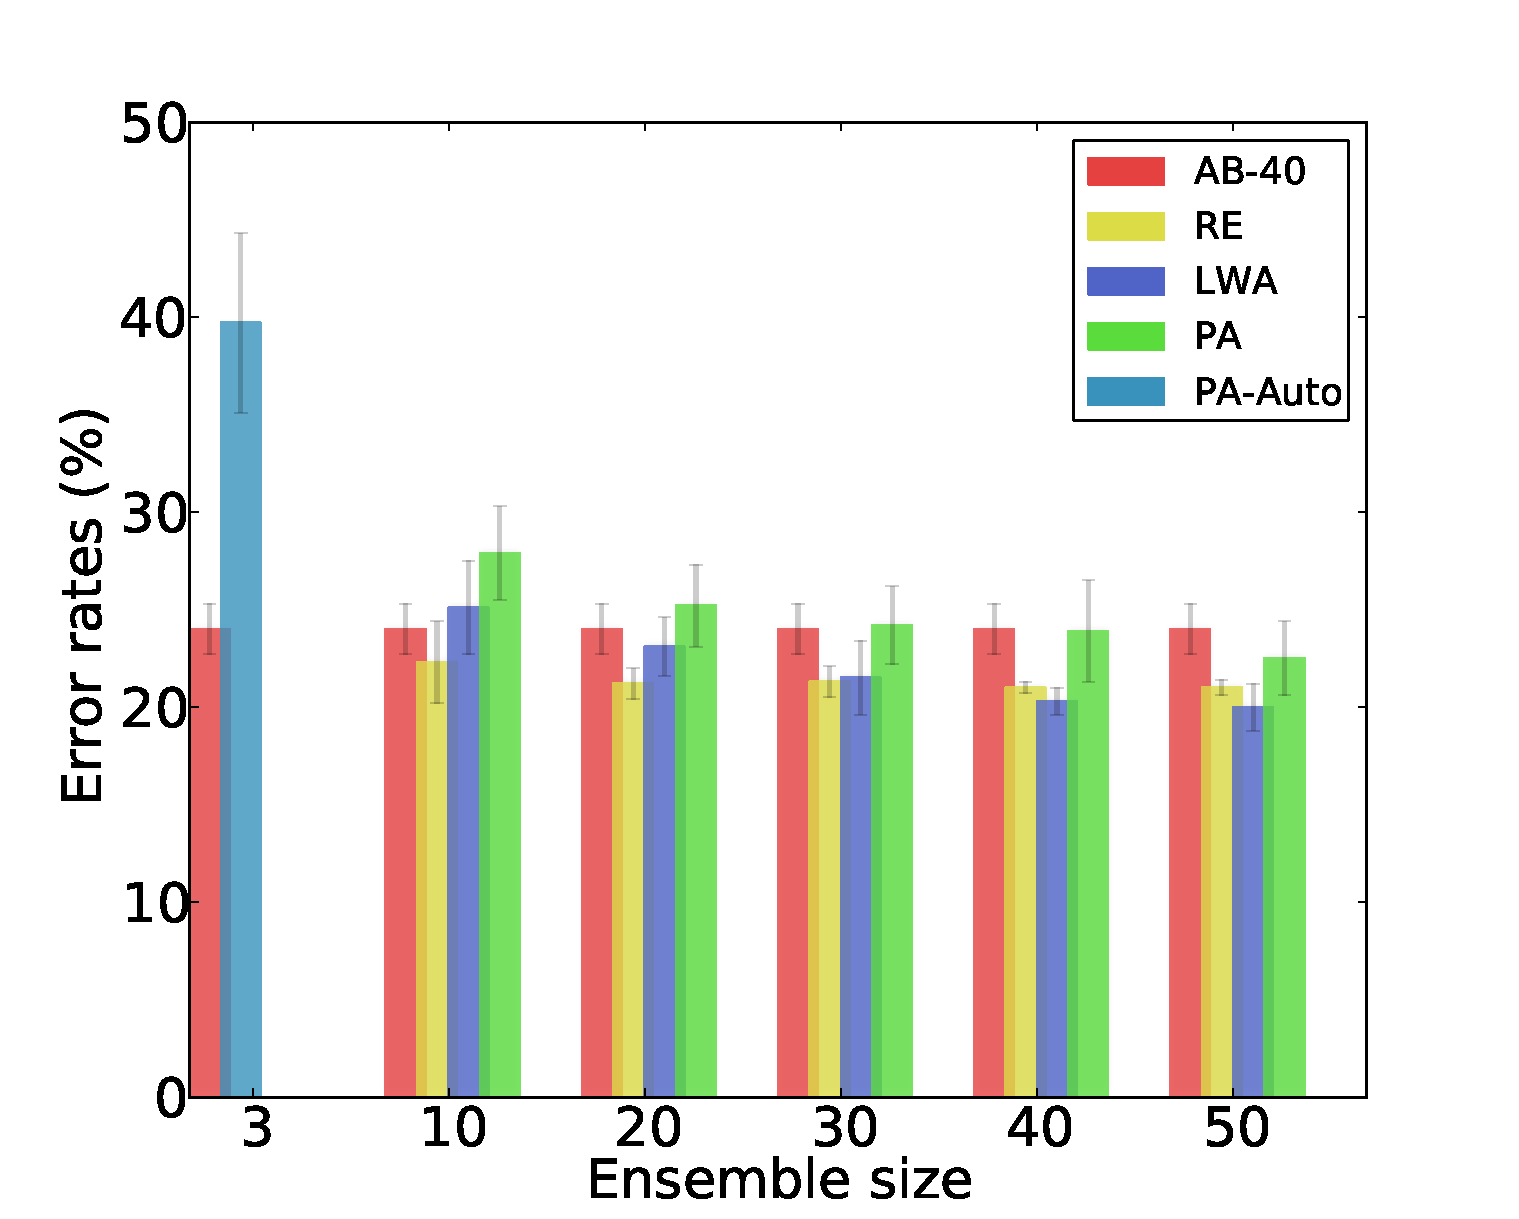
\includegraphics[width=0.3\linewidth]{results/drifts/extended/resultArtificial3MemPool}
            \end{block}
            \vfill
            \begin{block}{Results: Real World Datasets}
              \begin{itemize}
              \item Classifying real datasets with concept drifts, while the memory of previous stages are considered
              \end{itemize}
              \vskip-0.5ex
              
              \begin{table}
    \begin{center}
   %\footnotesize
   \footnotesize 	
   \centering
    \begin{tabular}{@{} l @{} r r r r }
    \cmidrule(l){2-5}
    &\multicolumn{4}{c }{ \# Ensemble Size}\\     
    \cmidrule(r){2-4}    \cmidrule(lr){5-5}
    &\multicolumn{3}{c }{10} &\multicolumn{1}{c }{50}\\
    \toprule
    \multicolumn{1}{ @{} l @{} }{\multirow{3}{*}{Real Data}} 			& \multicolumn{1}{c }{\multirow{3}{*}{\textit{LWA}}} & \multicolumn{1}{c }{\multirow{3}{*}{\textit{PA}}} & \multicolumn{1}{c }{\multirow{3}{*}{\textit{RE}}} & \multicolumn{1}{c }{\multirow{3}{*}{\textit{AdB}}}\\
    
   \multicolumn{1}{ @{} l @{} }{}& \multicolumn{1}{c }{} & \multicolumn{1}{c }{} & \multicolumn{1}{c }{} & \multicolumn{1}{c }{}\\      
    \cmidrule(r){1-1}     \cmidrule(lr){2-2}   \cmidrule(lr){3-3} \cmidrule(lr){4-4}   \cmidrule(lr){5-5} 
\multicolumn{1}{ @{} l @{} }{Sensor Streams \ \ \ \ \ \ \ \ \ \ } 			& \multicolumn{1}{r }{\ \ \ \  11.1 $\pm$ 5.0} & \multicolumn{1}{r }{\ \ \ \ 19.2 $\pm$ 9.7} & \multicolumn{1}{r }{\ \ \ \ \textbf{6.4 $\mathbf{\pm}$ 3.6}} & \multicolumn{1}{r }{\ \ \ \ 17.3 $\pm$ 9.7}\\     
\multicolumn{1}{ @{} l @{} }{Power Supply}			 & \multicolumn{1}{r }{28.3$\pm$0.2} & \multicolumn{1}{r }{28.3$\pm$0.2} & \multicolumn{1}{r }{\textbf{28.1$\mathbf{\pm}$0.0}} & \multicolumn{1}{r }{28.2$\pm$0.0}\\ 
\multicolumn{1}{ @{} l @{} }{Elec2}& \multicolumn{1}{r }{28.4$\pm$0.8} & \multicolumn{1}{r }{28.9$\pm$1.7} & \multicolumn{1}{r }{\textbf{27.3$\mathbf{\pm}$0.2}} & \multicolumn{1}{r }{30.5$\pm$3.9}\\ 
        \bottomrule
  \end{tabular}
    \end{center}
\end{table}
%
%              \begin{table}
%                \small
%                \centering
%                \begin{tabular}{@{} l @{} r r r r r r@{}}
%                  \toprule 
%                  Descriptor          & \multicolumn{6}{c @{}}{Error Rates [\%]}                                                                 \\
%                  \cmidrule(l){2-7}
%                  & \textit{AR1scarf}  & \textit{AR1sun}  & \textit{ARneutral} & \textit{AR2scarf} & \textit{AR2sun}  & Avg. \\
%                  \cmidrule(r){1-1}     \cmidrule(lr){2-2}   \cmidrule(lr){3-3} \cmidrule(lr){4-4}   \cmidrule(lr){5-5}  \cmidrule(lr){6-6}  \cmidrule(l){7-7} 
%                  SURF-64             & 2.72             & 30.00          & 0.00                & 4.54            & 47.27      & 16.90 \\        
%                  SURF-128            & 1.81             & 23.63          & 0.00                & 3.63            & 40.90      & 13.99 \\
%                  SIFT                & 1.81             & 24.54          & 0.00                & 2.72            & 44.54      & 14.72 \\
%                  \addlinespace
%                  U-SURF-64           & 4.54             & 23.63          & 0.00                & 4.54            & 47.27      & 15.99 \\
%                  U-SURF-128          & 1.81             & \textbf{20.00} & 0.00                & 3.63            & 41.81      & 13.45 \\
%                  U-SIFT              & \textbf{1.81}    & 20.90          & \textbf{0.00}       & \textbf{1.81}   & \textbf{38.18} & \textbf{12.54} \\
%                  \cmidrule(r){1-1}     \cmidrule(lr){2-2}   \cmidrule(lr){3-3} \cmidrule(lr){4-4}   \cmidrule(lr){5-5}  \cmidrule(lr){6-6}  \cmidrule(l){7-7}
%                  U-SURF-128+R        & 1.81             & 19.09          & 0.00                & 3.63             & 43.63     & 13.63 \\
%                  U-SIFT+R            & 2.72             & \textbf{14.54} & 0.00                & \textbf{0.90}    & 35.45     & 10.72 \\
%                  U-SURF-128+U-SIFT+R &  \textbf{0.90}   & 16.36          & \textbf{0.00}       & 2.72             & \textbf{32.72} & \textbf{10.54} \\       
%                  % \midrule 
%                  % \midrule 
%                  % DCT \cite{ekenel:facialocclusion:icb2009}, baseline%
%                  % & 8.2              & 61.8           & 7.3                & 16.4            & 62.7       & 31.28 \\
%                  % DCT \cite{ekenel:facialocclusion:icb2009}, realigned%
%                  % & 2.7              & 1.8            & 0.0                & 6.4             & 4.5        & 3.08  \\
%                  \bottomrule
%                \end{tabular}
%              \end{table}
            \end{block}
            \vfill
            \begin{block}{Conclusions}
              \begin{itemize}
              \item The selection of weak classifiers from different pools of sub-sampled data may improve the final ensemble in terms of accuracy, diversity and adaptation ability to drift. 
              \item The pruning method introduced in this research specially RE and LWA could improve the performance of AdaBoost in continuous learning and easily could be adapted for large datasets with high quantity of information. 
         
              \end{itemize}
            \end{block}
          }
          % ---------------------------------------------------------%
          % end the column
        \end{minipage}
      \end{beamercolorbox}
    \end{column}
    % ---------------------------------------------------------%
    % end the column
  \end{columns}
  \vskip1ex
  %\tiny\hfill\textcolor{ta2gray}{Created with \LaTeX \texttt{beamerposter}  \url{http://www-i6.informatik.rwth-aachen.de/~dreuw/latexbeamerposter.php}}
  \tiny\hfill{Created with \LaTeX \texttt{beamerposter}  \url{http://www-i6.informatik.rwth-aachen.de/~dreuw/latexbeamerposter.php} \hskip1em}
\end{frame}
\end{document}


%%%%%%%%%%%%%%%%%%%%%%%%%%%%%%%%%%%%%%%%%%%%%%%%%%%%%%%%%%%%%%%%%%%%%%%%%%%%%%%%%%%%%%%%%%%%%%%%%%%%
%%% Local Variables: 
%%% mode: latex
%%% TeX-PDF-mode: t
%%% End:
